\documentclass[10pt,pdf,hyperref={unicode}]{beamer} %aspectratio=169-для 16:9
\usepackage[T2A]{fontenc}
\usepackage[utf8]{inputenc}
\usepackage[english,russian]{babel} 
\usepackage{amssymb,amsfonts,amsmath,mathtext}
\usepackage{cite,enumerate,float,indentfirst}
\usepackage{graphicx}
\usepackage{movie15}
\usepackage{hyperref}

\graphicspath{{fig/}}

% Тема презентации
\usetheme[numbers, totalnumbers, minimal, nologo, nonav, compress]{Statmod}
%\usetheme{Singapore}
\usecolortheme{orchid}
%%%%%%%%%%%%%%%%%%%
%% Выбор шрифтов %%
\usefonttheme[onlylarge]{structurebold}

% Привычный шрифт для математических формул
\usefonttheme[onlymath]{serif}

% Более крупный шрифт для подзаголовков титульного листа
\setbeamerfont{institute}{size=\normalsize}
%%%%%%%%%%%%%%%%%%%

%%%%%%%%%%%%%%%%%%
%%% Сокращения %%%
% Синий цвет выделения
\setbeamercolor{color1}{bg=blue!60!black,fg=white}
%%%%%%%%%%%%%%%%%%

\title{ВЫПУСКНАЯ РАБОТА БАКАЛАВРА\\
\vspace{0.1cm}
Математическое моделирование течения трехфазной жидкости в пористых средах с использованием гибридных суперкомпьютеров}
\author{студент гр.871 Люпа А.А.}
\institute{Московский физико-технический институт \\
(государственный университет)\\
%\vspace{0.1cm}
Факультет управления и прикладной математики \\
Кафедра математического моделирования \\
    \vspace{0.2cm}
    Научный руководитель:  к.ф.-м.н. Чурбанова Н.Г.\\
}
\date{
    Москва 2012г.
}

% фоновый рисунок
%\usebackgroundtemplate{
\includegraphics[width=\paperwidth,height=\paperheight]{mipt-label.jpg}}

\begin{document}
\begin{frame}
  % создаём титульный лист
  \maketitle
\end{frame}

 \section{Введение}

 %% Цели и основные предположения
\begin{frame}
\begin{center}
\frametitle{Цели работы}
\begin{itemize}
\item {\large Построение модели течения трехфазных жидкостей в пористой среде, допускающей реализацию явными методами\\}
\vspace{0.5cm}
\item {\large Создание алгоритмов и программ, ориентированных на гибридные кластеры с графическими ускорителями\\}
\vspace{0.5cm}
\item {\large Проведение тестовых расчетов}
\end{itemize}
\end{center}
\end{frame}

 \section{Математическая модель}

% Основные предположения
\begin{frame}
\begin{center}
\frametitle{Основные предположения}
\begin{itemize}
\item Трехфазные течения: вода, легкая нефть и газ
\vspace{0.3cm}
\item Фазы несмешивающиеся
\vspace{0.3cm}
\item Жидкости слабосжимаемые
\vspace{0.3cm}
\item Газ идеальный
\vspace{0.3cm}
\item Среда пористая, однородная, изотропная, неподвижная
\vspace{0.3cm}
\item Учитываются капиллярные силы и гравитационное поле
\vspace{0.3cm}
\item Не учитываются тепловые процессы
\end{itemize}
\end{center}
\end{frame}

%% Математическая модель
\begin{frame}
\begin{center}
\frametitle{Математическая модель}
Полная система уравнений для описания трехфазных течений
при сделанных предположениях:
\begin{equation*}
\left\{
  \begin{aligned}
    &\overrightarrow{u_i}=-K \frac{k_i(S_i)}{{\mu}_i}(grad P_i - {\rho}_i\overrightarrow{g})\\
    &m\frac{\partial (\rho_i S_i)}{\partial t}+ div(\rho_i \overrightarrow{u_i}) = 0 \\
    &{\rho}_i = {\rho}_i(P_i) \\
    &i=w,n,g\\
    &P_n=P_w+P_{cnw}(S_w)\\
    &P_g=P_w+P_{cnw}(S_w)+P_{cgn}(S_g)\\
    &S_w + S_n + S_g=1
  \end{aligned}
\right.
\end{equation*}
В качестве независимых переменных выбраны $S_w$, $S_n$, $P_w$.
\end{center}
\end{frame}

\section{Алгоритм расчетов}

%% Алгоритм расчетов
\begin{frame}
\begin{center}
\frametitle{Алгоритм расчетов}
\begin{enumerate} 
\item Вычисление давлнений $P_n$,
$P_g$ через $P_w$ и капиллярные давления. 
\item Вычисление плотностей фаз. 
\item
Нахождение относительных фазовых проницаемостей фаз. 
\item Вычисление скоростей
фаз независимо по всем измерениям. 
\item 
\label{roS} 
Нахождение ${\rho}_iS_i$ на
следующем шаге по времени из уравнения неразрывности явным численным методом.
\item 
\label
{Newton} Решение системы трех нелинейных уравнений методом Ньютона,
в результате чего находим $P_w$, $S_w$, $S_n$ на следующем шаге по времени.
\item Применение граничных условий. 
\item Сохранение полученных значений переменных в текстовый файл
в формате, подходящем для визуализации(если нужно).
\item Обмены данными при многопроцессорных вычислениях.
\end{enumerate} 
\end{center}
\end{frame}

\section{Программная реализация}

%% Комплекс программ для моделирования процессов в подземном пространстве на гибридных суперкомпьютерах
\begin{frame}
\begin{center}
\frametitle{Комплекс программ для моделирования процессов в пористых средах на гибридных суперкомпьютерах}
\begin{itemize}
\item Задачи в прямоугольных областях
\item Ортогональные расчетные сетки
\item Логически простые алгоритмы на основе явных разностных схем
\item Геометрический параллелизм, равномерная балансировка загрузки и обмен данными на внутренних границах подобластей
\item Язык программирования С/C++, технологии CUDA и MPI
\item Модульная структура (вычислительные, коммуникационные и управляющие модули)
\item Расчеты 2D и 3D задач
\item Кроссплатформенность(Windows и Linux)
\item Возможность задействовать любое число CPU и GPU
\item Оптимизация доступа к различным типам памяти
\end{itemize}
\end{center}
\end{frame}

\section{Тестовые расчеты}

\begin{frame}
\frametitle{Задача перераспределения фаз}
\begin{center}
 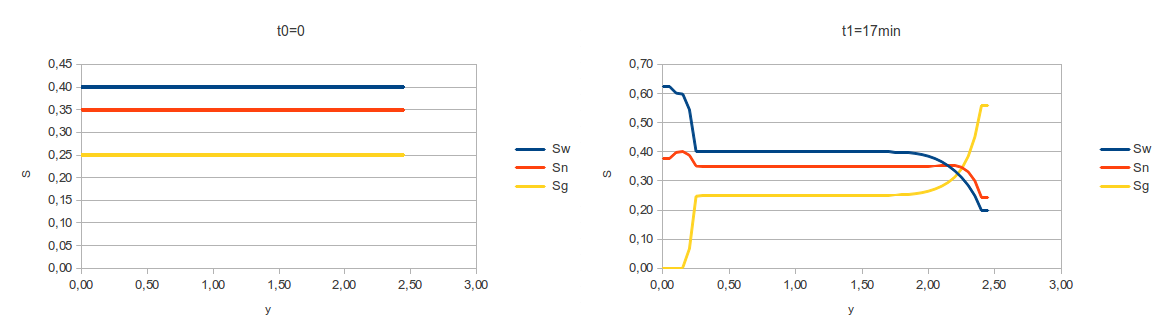
\includegraphics[width=8.5cm,height=3.5cm]{test1_1}
\end{center}
\begin{center}
 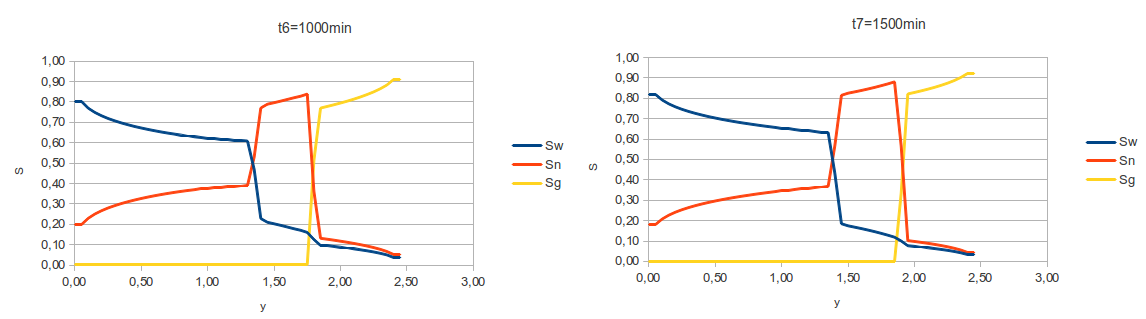
\includegraphics[width=8.5cm,height=3.5cm]{test1_4}
\end{center}
\begin{center}
 %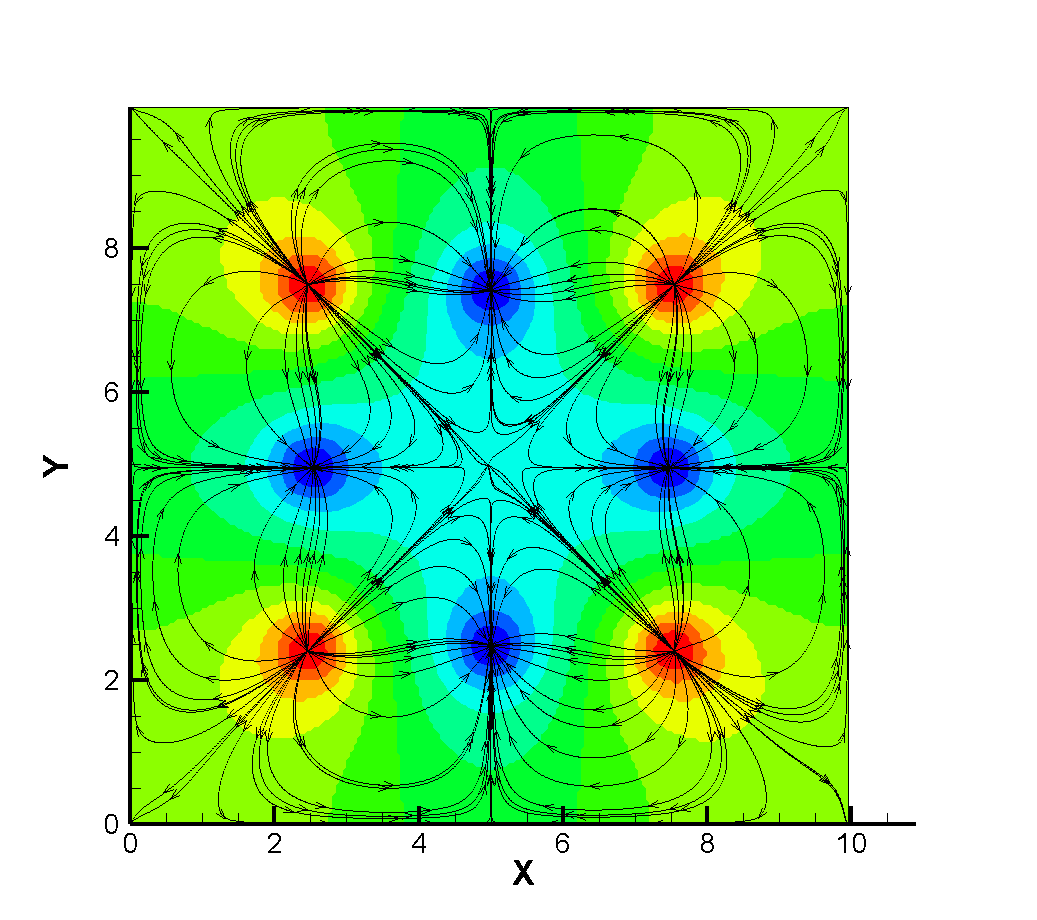
\includegraphics[width=12cm,height=11cm]{test3}
\end{center}
\end{frame}


\begin{frame}
\frametitle{Задача просачивания}
\begin{center}
 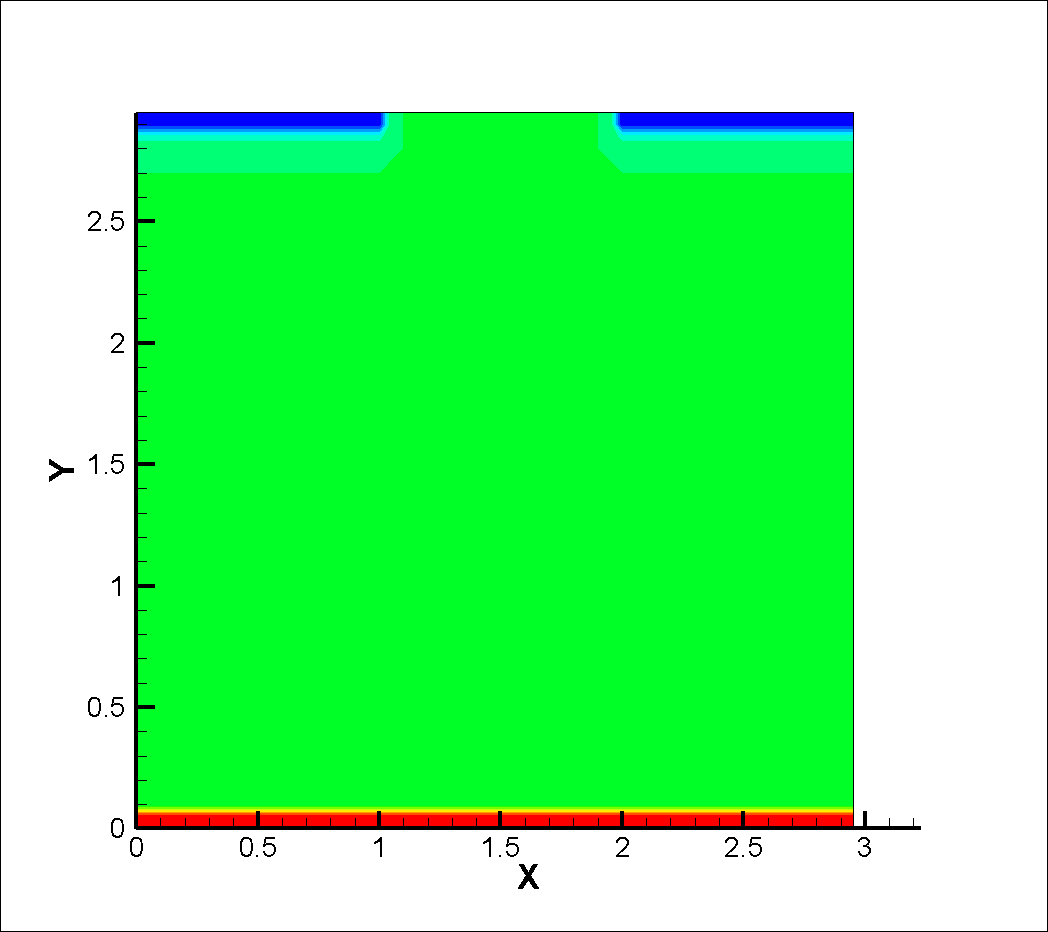
\includegraphics[width=3cm,height=3cm]{test2_1Sw}
 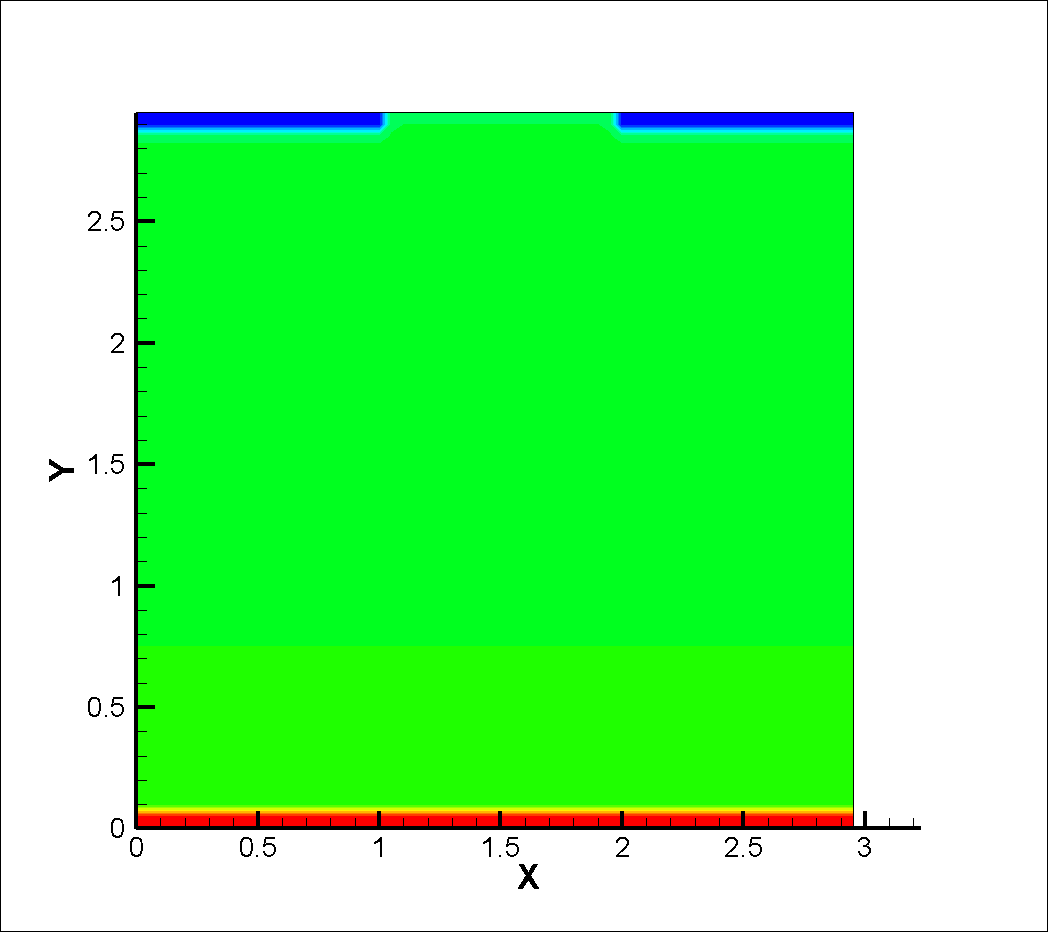
\includegraphics[width=3cm,height=3cm]{test2_1Sn}
 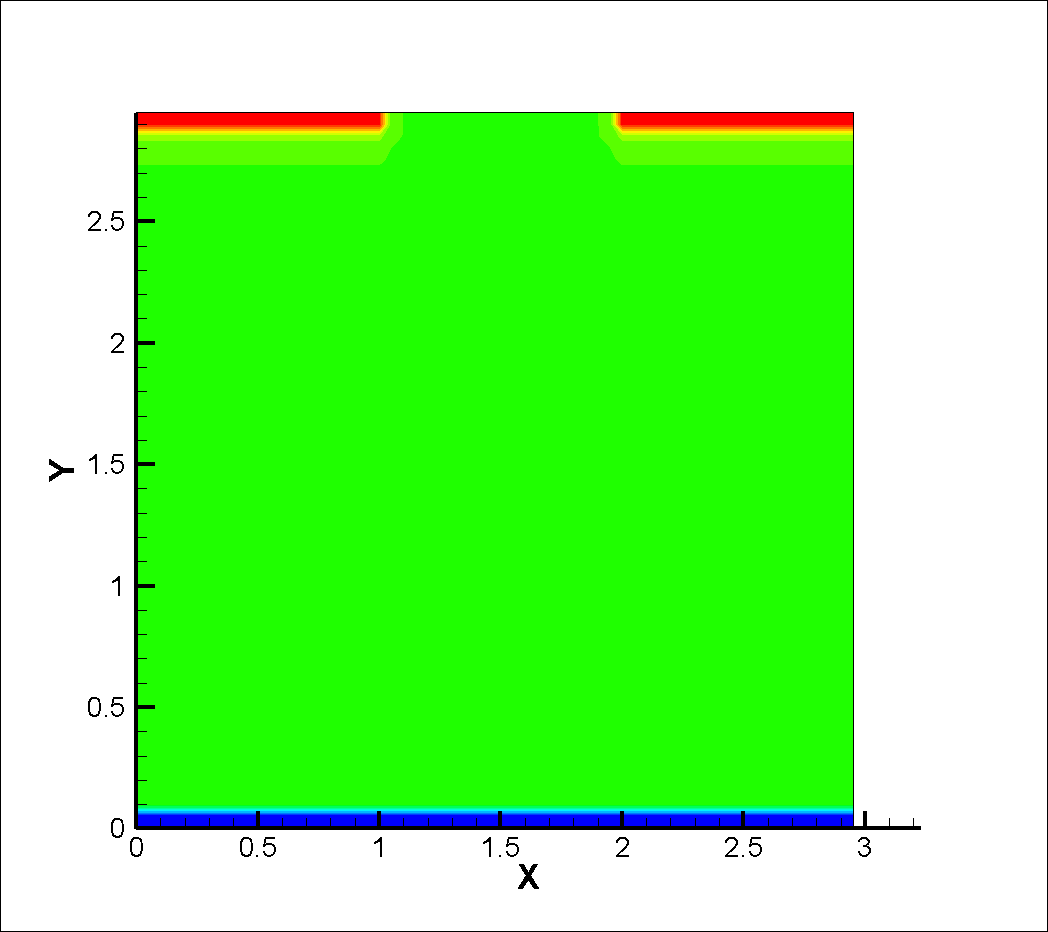
\includegraphics[width=3cm,height=3cm]{test2_1Sg}
\end{center}
\begin{center}
  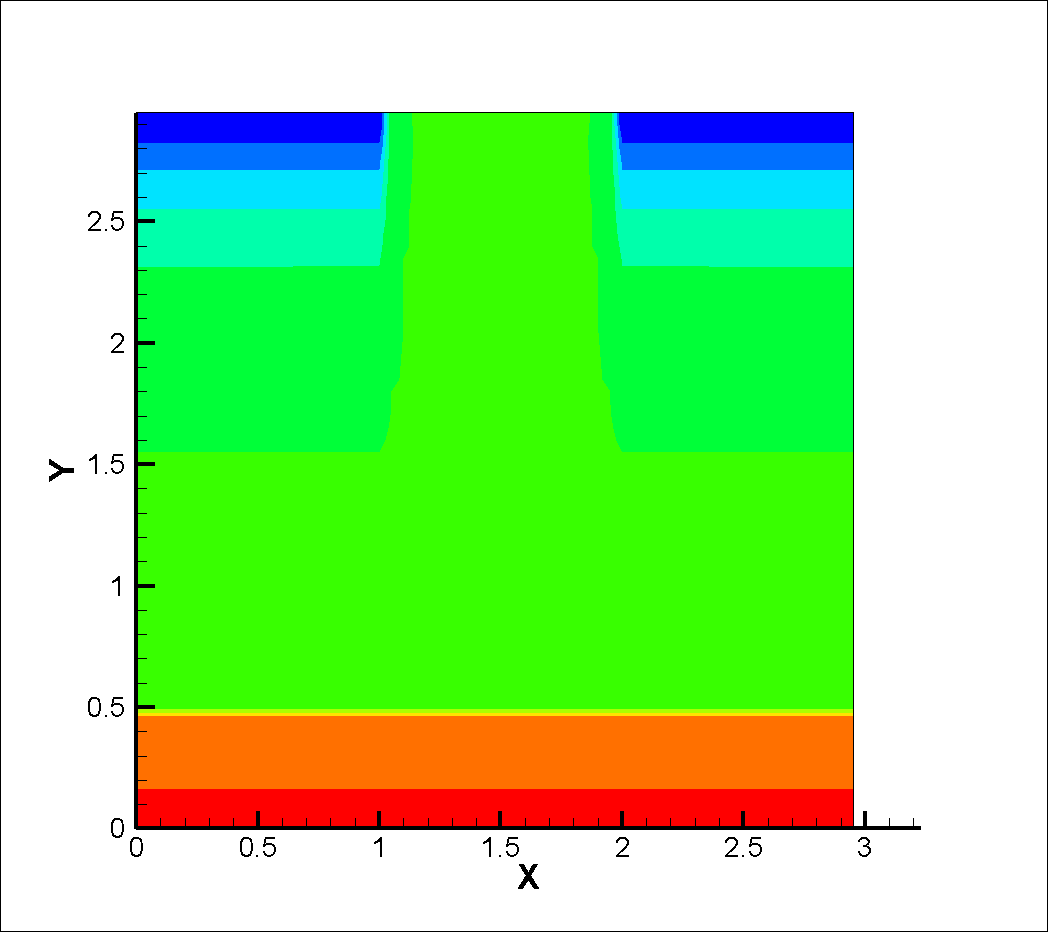
\includegraphics[width=3cm,height=3cm]{test2_4Sw}
 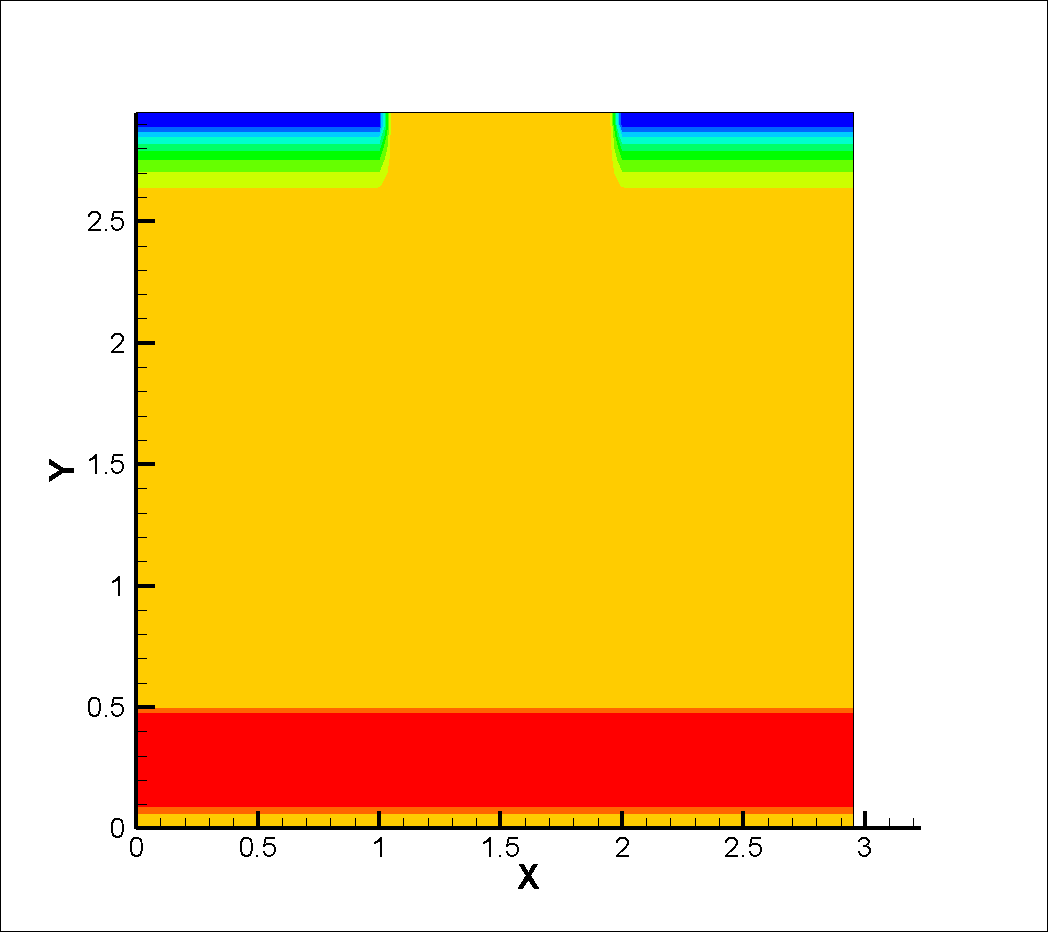
\includegraphics[width=3cm,height=3cm]{test2_4Sn}
 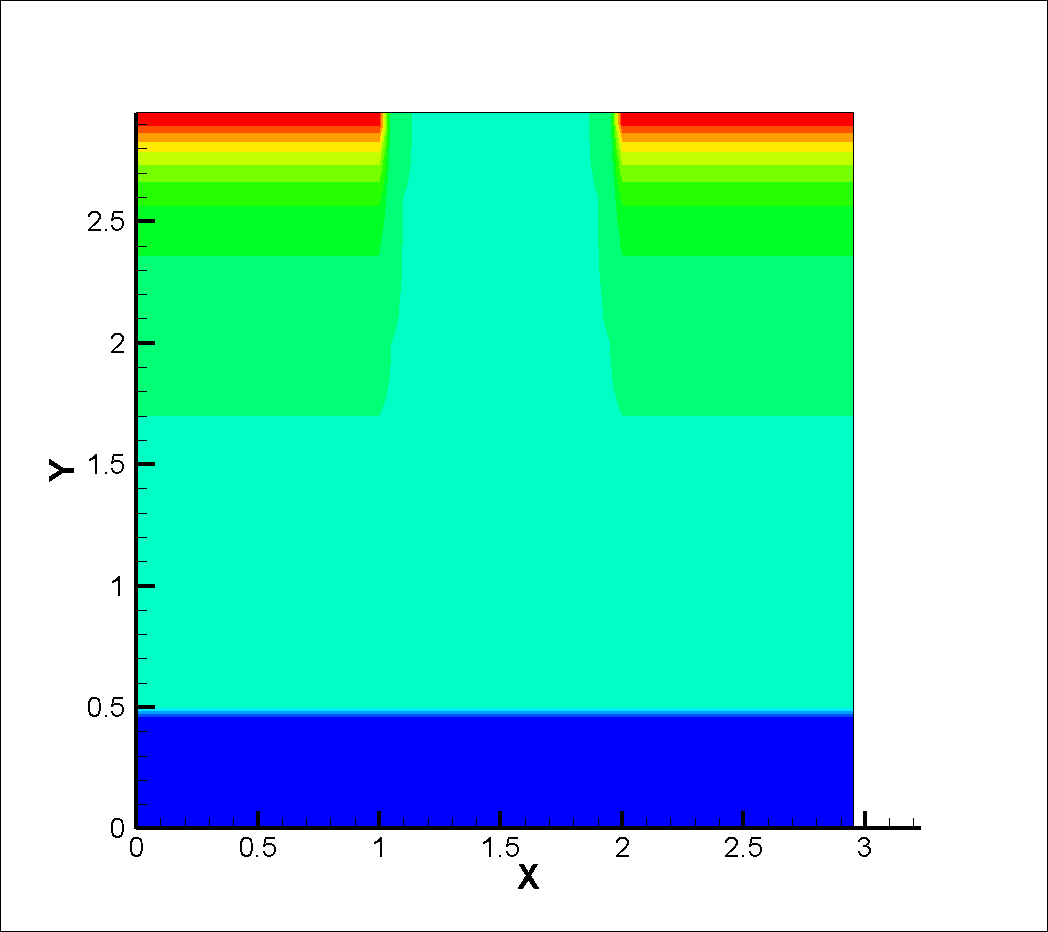
\includegraphics[width=3cm,height=3cm]{test2_4Sg}
\end{center}
\begin{center}
 %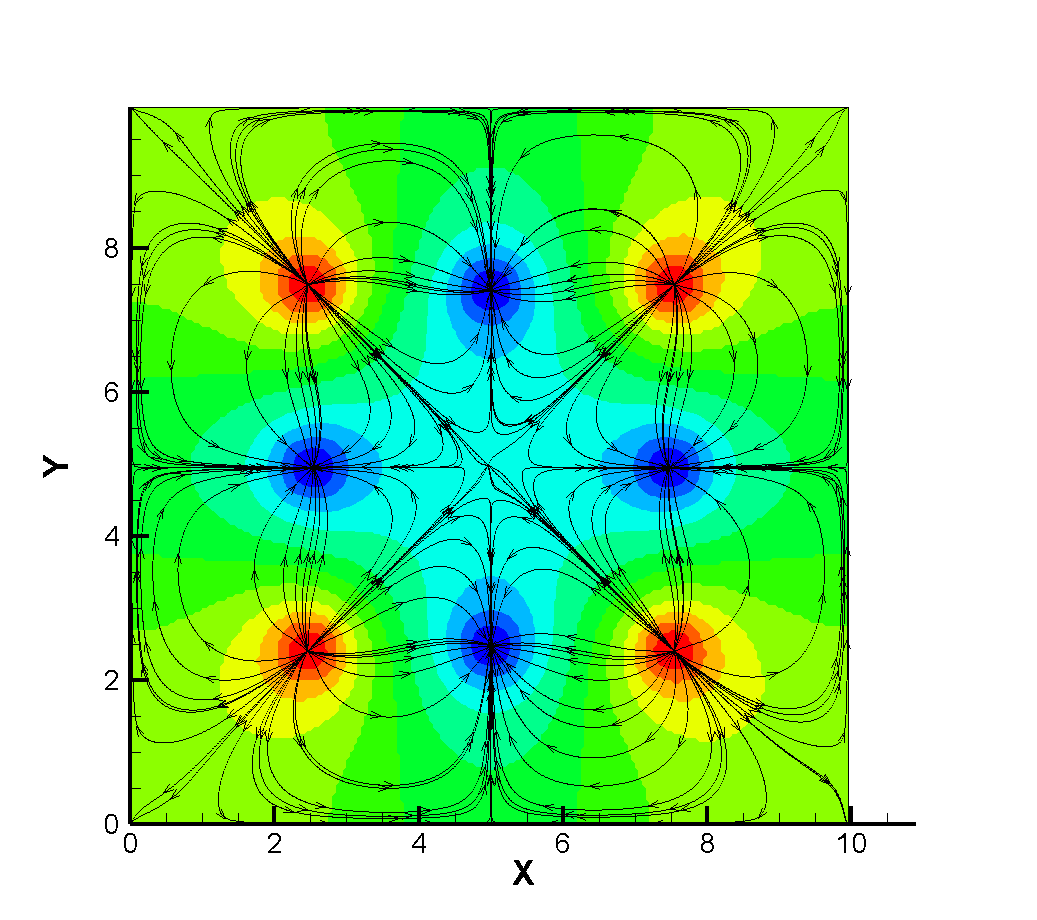
\includegraphics[width=12cm,height=11cm]{test3}
\end{center}
\end{frame}

%% Тестовые расчеты
\begin{frame}
\begin{center}
\frametitle{Задача нефтедобычи}
\begin{center}
 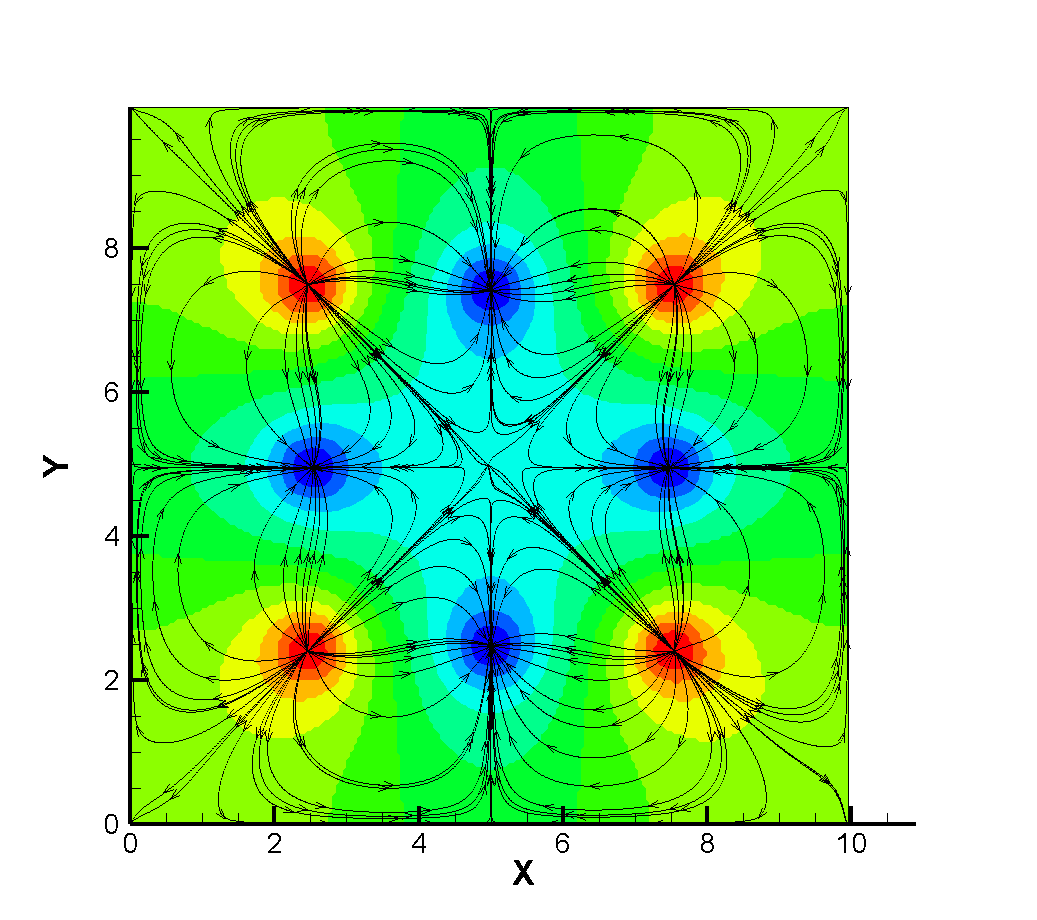
\includegraphics[width=8cm,height=7.5cm]{test3}
\end{center}
\end{center}
\end{frame}

\begin{frame}
\begin{center}
\frametitle{Результаты совместного применения библиотек CUDA и MPI}
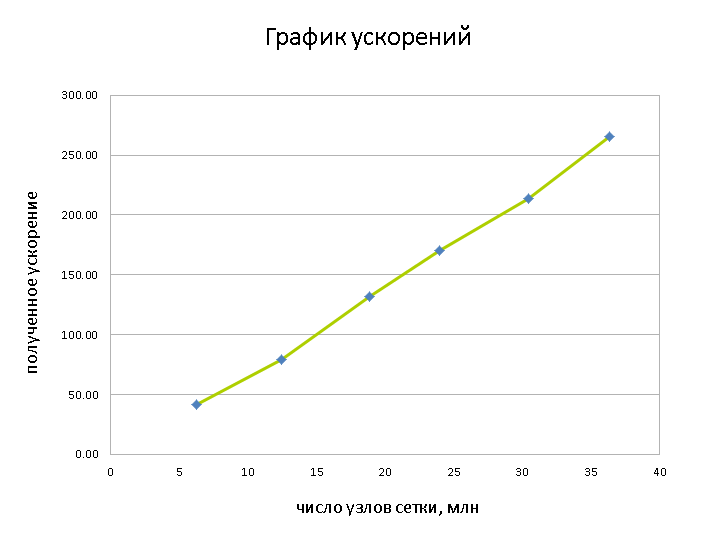
\includegraphics[width=8cm]{sgpu.png} 
\end{center}
\end{frame}

\section{Заключение}
%% В дальнейшем планируется:
\begin{frame}
\begin{center}
\frametitle{Заключение}
{\Large В дальнейшем планируется:}
\vspace{1.0cm}
\begin{itemize}
\item	{\large ставить и решать задачи трехфазной фильтрации в
	неоднородных, анизотропных средах;}		
\vspace{0.5cm}
\item 	{\large улучшить геометрическое деление области при многопроцессорных
	вычислениях;}
\vspace{0.5cm}
\item 	{\large оптимизировать использование графических плат;}
\vspace{0.5cm}
\item 	{\large применить разностные схемы с лучшими свойствами.}
\end{itemize}
\end{center}
\end{frame}

%% Спасибо за внимание
\begin{frame}
\begin{center}
\frametitle{}
\item {\huge Спасибо за внимание!}
\end{center}
\end{frame}

\end{document}
